% !TeX root = ../thesis.tex
%*****************************************************************************************
%*********************************** Forth Chapter ***************************************
%*****************************************************************************************
\chapter{On relationships with an active longitude}\label{ch:4}  %Title of the Second Chapter

\begin{pycode}[chapter4]
from __future__ import print_function

ch4 = texfigure.Manager(pytex, number=4, base_path='./Chapter4/')
\end{pycode}

\section{Introduction}
Studies of non-uniform distribution of solar activity began with \cite{Chidambara1932}.
Investigations of sunspot groups distribution finds that they tend to cluster towards a certain heliographic longitude [\cite{Bumba1965,Balthasar1984,Wilkinson1991}].
These authors present the concept of an active longitude, at which sunspot groups cluster.
As the field advanced, studies have presented the same concept applied to a range of solar features, \cite{Zhang2007} demonstrated this behaviour with solar flares.
\cite{Benevolenskaya1999} demonstrate a clustering in surface magnetic fields, and, \cite{Mursula2004} present active longitudes in the heliospheric magnetic field.
Lastly, and most applicably to this work, \cite{Jing2011} have observed this to be case in coronal streamers.

\newpage
Macrospicules (hereinafter: MS) are chromospheric objects observed in H$\alpha$ and He $30.4$ nm \cite{Bohlin1975,Wang199 8,Murawski2011,Scullion2010}. 
They are explosive jet-like features extending up to, on average, $29$ Mm and velocities up to approximately $110$ km/s \cite{Zaqara_Erdelyi2009}. 
Their structure reflects the solar atmosphere they move through, they are proposed to have a cool core, surrounded by a hot sheath \cite{Parenti2002}. 
They are of particular use in this study, as they are observed from the solar equator to the poles. 

This chapter will discuss the longitudinal and latitudinal distributions of MS.
Extending this, we will compare the behaviour of MS to those already observed in the studies highlighted above, particularly solar active regions.

\section{Observations and Databases}
The MS were observed using the $30.4$ nm SDO/AIA [\cite{AIAspec}]. 
This takes a $4096 \times 4096$ pixel, full disc, image of the Sun at a cadence of $12$ s. 
We took typical samples of two hours, twice a month, from June $2010$ until December $2012$.
For each image the solar limb was flattened out, making it easier to identify and measure the MS.
They are extremely difficult to measure on disk, and as such, this study concentrates on those occurring at the limb.
We record the time at the moment they become visible at the limb and their angular displacement from solar due east.
Measuring MS this way we identified 101 examples of MS. The physical dimensions and the heliographic coordinates have been estimated. 

Debrecen Photoheliographic Data (DPD) sunspot catalogue [\cite{Gyori2011}] has been used as the source of sunspot groups used to calculate the most prevalent active longitudes.
This database builds on from the Greenwich Photoheliographic Results (GPR), which bas been the basis of many works in the field.
DPD has been used to provide a sample beginning in $1974$, detailing every sunspots area and position since that epoch.

\section{Statistical Study of the Latitudinal Distribution of MS}
In order to examine the spatial behaviour of MS we must determin the heliographical latitudes (B).
In order to aid analysis, the Carrington latitudes, $B$, have been transformed into the following system:

\begin{equation}
\begin{split}
\phi=-(B+90^{\circ})/90^{\circ},  B<0 \\
\phi=-(B-90^{\circ})/90^{\circ},  B>0
\end{split}
\end{equation}

The domain of interest of the quantity $\phi$ is $[-1;1]$. 
The $\phi=0$ point contains the northern and southern poles.
The $[0;1]$ sub-domain of $\phi$ represents the northern hemisphere, the ascending $\phi$ values from $0$ to $1$ show the descending latitudes from $90^{\circ}$ to $0^{\circ}$. 
The southern hemispheres have been considered in the same way.

Figure~\ref{ms_dis} shows the result of the statistics above. 
The histogram depicts a normal distribution. 
$\overline{\phi}=0.043$, this implies that most of the MS tend to cluster to the poles, as has previously been shown to be the case in \ref{ch:3}, confirming the method.
We also find that the northern hemisphere was a slightly more active in this time period.
The standard deviation values are $1\sigma=0.3507$ and $2\sigma=0.7014$. 
Hence, $68\%$ of MSs measured in this data set, cluster in a $31.5^{\circ}$ wide belt from the poles.
The extension of this is that $68\%$ of MS are between the $\pm58.5^{\circ}$ and $\pm90^{\circ}$ heliographic latitude, and, $95\%$ of MS are in a $36^{\circ}$ degree belt from the poles or between $\pm27^{\circ}$ and $\pm90^{\circ}$ in heliographic latitude.
Demonstrating that MS exhibit longitudinal inhomogeneity at higher latitudes.

\begin{figure}
	\centering
	{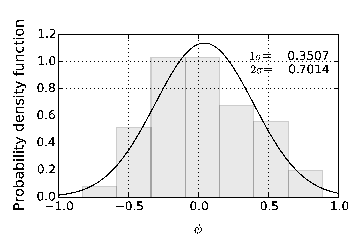
\includegraphics[width=0.6\textwidth]{Chapter4/Figs/MS_latitude_distribution}}
	{\caption{ The gray area shows the probability density function of the parameter $\phi$. The solid black line is the fitted Gaussian distribution. The values standard deviation $1\sigma$ and $2\sigma$ of the normal distribution have been indicated in the top right corner.}\label{ms_dis}}
\end{figure}

\section{Statistical study of longitudinal distribution of MS}
\subsection{Activity maps of active longitudes based on sunspots}

According to \cite{Gyenge2014}, the method highlighted above has been proven and the active longitude was found to be distinct in each hemisphere.
The present investigation started with a similar method as described in \cite{Gyenge2012}. 
In to construct a complete picture of the active longitudes when considering sunspots, the areas and positions of all sunspot groups are included in this analysis.
The solar surface is divided into longitudinal bins of $20^{\circ}$ and the areas of all groups were summed up in each bin: $ A_{i}$ in certain Carrington Rotation between $2097$ and $2128$, the temporal sample over which the MSs locations was recorded.
Next, the longitudinal activity concentration is represented by the quantity $W$ defined by:

\begin{equation}
W_{i,CR} = \frac{A_{i,CR}}{ \sum_{j=1}^{N} A_{j,CR} },
\end{equation}

where $N$ is the number of bins, $\sum_{j=1}^{N} A_{j,CR}$  is the sum of all sunspot groups in a given CR and $A_{i,CR}$ is the  total area of sunspot groups in a Carrington Rotation and at a specific longitudinal bin.

In each Carrington Rotation we omitted all of the $ W_{i,CR}$ values which are lower than the $3\sigma$ significance limit.
The highest peak, inferred as the active longitude in the Carrington Rotation co-ordinate frame, $AL_{CR}$, has been selected from this decayed sample (which contains only the significant peaks) caused by the significance test.
For further analysis, the Carrington longitudes, $\lambda$, will now be transformed, into Carrington phase period: 

\begin{equation}
\psi = \lambda/360^{\circ}.
\end{equation}

Hence, the values of the phases are always smaller or equal (which is the entire circumference) than one. 

The time-variation of the parameter $AL_{CR}$ is plotted in Figure~\ref{AL}.
The vertical axis is the phase parameter, which has been repeated $3$ times.
The northern (left-hand-side) and the southern (right-hand-side) cases are considered separately. Both figures unveil a clear increasing migration pattern. \cite{Usoskin2005,Gyenge2014} found similar patterns at a different time interval. Most of the migration follows a parabola shape (which has been fitted by the least-square method).

\begin{figure}
	\centering
	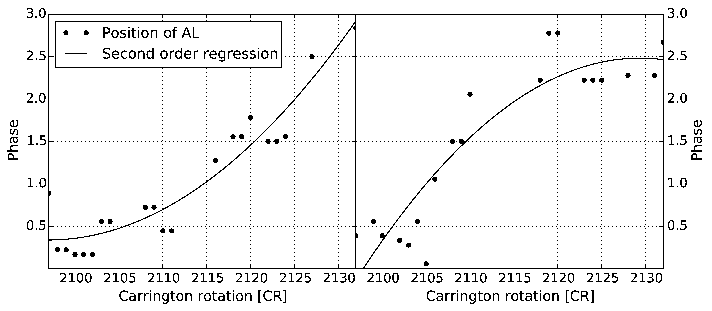
\includegraphics[width=128mm]{Chapter4/Figs/AL}
	\caption{The migration of the active longitudes in the time interval of CR $2097$ to $2128$ based on sunspot groups. The left panel sows the northern hemisphere. The right panel is the southern hemisphere.}
	\label{AL}
\end{figure}

\subsection{Relationship between the AL and MS longitudinal distribution}

\begin{figure}
	\centering
	{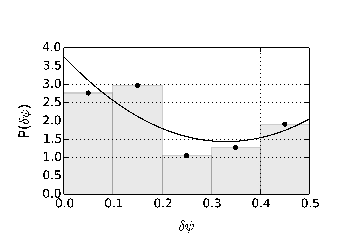
\includegraphics[width=90mm]{Chapter4/Figs/stat}}
	{\caption{Density distribution of the $\delta\psi$ parameter. }\label{stat}}
\end{figure}	

The parameter $\delta\psi$ is now introduced to study the relationship between the active longitude, $AL_{CR}$, defined by sunspot groups, and the longitudinal position of MS $L_{CR}$ in Carrington Rotation co-ordinates. 

\begin{equation}
\delta\psi = \left| AL_{CR} - L_{CR}\right|.
\end{equation}

The parameter $\delta\psi$ has been reduced by a unit phase if it is larger than $0.5$, which means this quantity represents the shortest phase difference between the longitudinal position of a given MS and the position of active longitudes in both hemispheres. 
Next, the $\delta\psi$ samples of the northern and southern hemispheres are now combined. 

The probability density function (PDF) of the quantity $\delta\psi$ is shown in Figure~\ref{stat}. On the $x$-axis the meaning of the lower values reflect on the smallest longitudinal difference in phase, the value $0.5$ phase jumps to the opposite side of the Sun.

The domain of interest of the quantity $\phi$ is $[-1;1]$. 
The $\phi=0$ point contains the northern and southern poles.
The $[0;1]$ sub-domain of $\phi$ represents the northern hemisphere, the ascending $\phi$ values from $0$ to $1$ show the descending latitudes from $90^{\circ}$ to $0^{\circ}$. 
The southern hemispheres have been considered in the same way.

Figure~\ref{ms_dis} shows the result of the statistics above. 
The histogram depicts a normal distribution. 
$\overline{\phi}=0.043$, this implies that most of the MS tend to cluster to the poles

The MS tend to cluster near the active longitudes, which is shown by the first and second peaks: $\delta\psi< 0.2 (<\pm 36^{\circ}$) 61 \% of the candidates.
However, there is a significant peak around $0.5$, which is the signature of the appearance of secondary longitudinal belts. 
The secondary belt exists alongside the primary belt temporally. 
It is always the case that the primary belt is always stronger than the secondary belt, as the name implies), and the phase shift is around $0.5$.
The MS show a similar behaviour, a secondary belt appears for $22\%$ of the events and $\delta\psi< 0.1 (<\pm 18^{\circ}$).

\section{Summary}
We investigated the distribution of MSs detected at the solar surface as function of their longitudinal and latitudinal coordinates in Carrington co-ordinates.

A non-homogeneous latitudinal macrospicule distribution has been found. 
The macrospicules are found to have a non-homogeneous distribution in the Carrington co-ordinate frame.  
Most of the events tend to cluster to the higher latitudes ($95\%$ of MS are with in the $\pm27^{\circ}$ to $\pm90^{\circ}$ heliographical latitude).
The number of the events is found to be growing exponentially from the equator to the pole in both hemispheres. 
A slightly asymmetrical behaviour has been found between the two hemispheres in the studied time interval, where the northern hemisphere was marginally more active than the southern. 

The latitudinal spatial distribution of MS is not uniform either. A large proportion of the MS (83 of from the 101 in our sample) tend to cluster to the AL.
In the case of the primary active longitude belt, the MSs are within $\pm 36^{\circ}$ degrees of the active longitude.
The secondary belt has a $\pm 18^{\circ}$ wide range within which the MSs are found to be concentrated.
This supports the existence of an active longitude at higher latitudes.

A large sample and more comprehensive statistical study is now in preparation for a more detailed search for further identifiable non-homogenous longitudinal distributions of MS in the entire time period covered by observations of the SDO satellite.
